\documentclass{article}

\usepackage{tikz}

\begin{document}

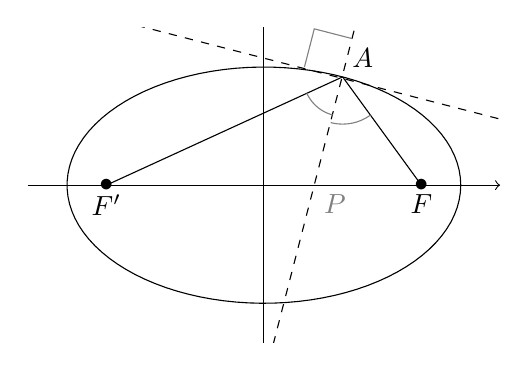
\begin{tikzpicture}[scale=0.5]
  \clip (-6,-4) rectangle (6,4);
  % axes
  \draw[->] (-6,0) -- (6,0);
  \draw[->] (0,-4) -- (0,6);
  % ellipse
  \draw plot [samples=100,domain=0:360] ({5 * cos(\x)},{3*sin(\x)});
  % foyer F
  \draw (4,0) node{$\bullet$} coordinate (f1) node[below]{$F$};
  % foyer F'
  \draw (-4,0) node{$\bullet$} coordinate(f2) node[below]{$F'$};
  % A sur l'ellipse
  \draw (2,2.75) coordinate (a) node[above right] {$A$};
  \draw (a) -- (f1); % rayon focal (AF)
  \draw (a) -- (f2); % rayon focal (AF')
  % tangente en A
  \draw [dashed] plot [domain=-6.5:6.28](\x,{(1.24-0.97*\x)/-0.25});
  % normale en A
  \draw [dashed]  plot [domain=-6.5:6.28](\x,{(1-0.08*\x)/0.31});
  \coordinate (p) at (1.28,0) ; % P point de la normale sur Ox
  \draw (p) node[below right,gray]{$P$}; 
  \begin{scope} % scope pour clip
    \clip (a) -- (p) -- (f2) -- cycle; % triangle APF'
    \draw [gray] (a) circle (1); % cercle pour arc
  \end{scope}
  \begin{scope} % scope pour clip
    \clip (a) -- (p) -- (f1) -- cycle; % triangle APF
    \draw [gray]  (a)  circle (1.2); % cercle pour arc
  \end{scope}
  \draw [gray] (2.25,3.72) -- (1.28,3.97) -- (1.03,3); % angle droit en A
\end{tikzpicture}

\end{document}
